\documentclass[11pt]{article}
%\baselineskip 16pt
\usepackage{amsmath}
\usepackage{amssymb}
\usepackage{graphicx}
\usepackage{qcircuit}
\usepackage{upquote}
\usepackage{array}

\setlength{\oddsidemargin}{-0.15in}
\setlength{\topmargin}{-0.5in}
\setlength{\textheight}{9in}
\setlength{\textwidth}{6.5in}

\newtheorem{theorem}{Theorem}[section]
\newtheorem{definition}[theorem]{Definition}
\newtheorem{proposition}[theorem]{Proposition}
\newtheorem{corollary}[theorem]{Corollary}
\newtheorem{lemma}[theorem]{Lemma}
\newtheorem{example}[theorem]{Example}
\newtheorem{remark}[theorem]{Remark}
\def\qed{\hfill $\Box$\medskip}

\def\IR{{\mathbb R}}
\def\IC{{\mathbb C}}
\def\IF{{\mathbb F}}
\def\II{{\mathbb I}}
\def\IN{{\mathbb N}}
\def\IQ{{\mathbb Q}}
\def\IZ{{\mathbb Z}}
\def\cE{{\mathcal E}}
\def\ra{{\rangle}}
\def\la{{\langle}}
\def\cS{{\cal S}}
\def\cB{{\cal B}}
\def\cR{{\cal R}}
\def\cP{{\cal P}}
\def\cF{{\cal F}}
\def\bC{{\bf C}}
\def\bP{{\bf P}}
\def\bM{{\bf M}}
\def\bd{{\bf d}}\def\({\left (}
\def\){\right )}
\def\logm{{\prec_{\rm log}}\,}
\def\diag{{\rm diag}\,}
\def\tr{{\rm tr}\,}
\def\rank{{\rm rank}\,}
%\def\span{{\rm span}\,}
\def\dfrac{\displaystyle\frac}


\def\ket#1{| #1 \rangle}
\def\bra#1{\langle #1 |}
\def\kb#1#2{|#1\rangle\!\langle #2 |}
%\pagestyle{empty}
\begin{document}
\openup 1\jot

\title{Error correlation schemes for fully correlated quantum channels
protecting both quantum and classical information}


\author{Chi-Kwong Li, Seth Lyles, Yiu-Tung Poon}
\date{}
\maketitle
\begin{abstract}
We study efficient quantum error correction schemes
for the fully correlated channel on an
$n$-qubit system with error operators
that assume the form $\sigma_x^{\otimes n}$, $\sigma_y^{\otimes n}$, 
$\sigma_z^{\otimes n}$.
In particular, when $n=2k+1$ is odd, we describe a quantum error correction scheme 
using one arbitrary qubit $\sigma$
to protect the data state $\rho$ in the $2k$-qubit system
such that only $3k$ CNOT gates (each with one control bit and one target bit) 
are needed
to encode the $n$-qubits. The inverse operation of the CNOT gates
will produce $\tilde \sigma \otimes \rho$, so a partial 
trace operation can recover $\rho$.
When $n = 2k+2$ is even, we describe a hybrid quantum error correction scheme
that protects a $2k$-qubit state $\rho$
and 2 classical bits encoded as $\sigma \in \{|ij\ra \la ij|: i, j \in \{0,1\}\}$;
the encoding can be done by $3k+2$ CNOT gates and a Hadamard gate on one qubit,
and the inverse operation will be the decoding operation producing 
$\sigma \otimes \rho$.
The scheme was implemented using Matlab, Mathematica and
the IBM's quantum computing framework \verb|qiskit|.

\end{abstract}

\noindent
\section{Introduction}


In quantum information processing, information is stored and processed
with a quantum system. In the mathematical setting,  quantum states are
represented as density matrices, i.e., complex positive semi-definite matrices
with trace one. Denote by $D_N$ the set of density matrices in the set 
$M_N$ of $N\times N$ complex matrices. A qubit will be represented as a
matrix in $D_2$, and a quantum state of an $n$-qubit system will be a matrix
in $D_N$ with $N = 2^n$.
A quantum channel on an $n$-qubit system is a
trace preserving completely positive linear map
$\cE: M_N\rightarrow M_N$ that admits the operator sum representation
$$\cE(\rho) = \sum_{j=1}^r F_j \rho F_j^\dag  \qquad \hbox{ for all } \rho \in M_N,$$
where $\sum_{j=1}^r F_j^\dag F_j = I_N$. The matrices $F_1, \dots, F_r$ are sometimes 
called the error operators of the quantum channel $\cE$, which is the source of the
corruption of the quantum states corresponding to decoherence and other quantum effect
on the quantum state $\rho$. To protect the information stored in the quantum state
$\rho$, one can use quantum error correction schemes to encode the
quantum state $\rho$ with some auxiliary qubits $\rho$  
so that one can recover the quantum state $\rho$ after the encoded 
quantum state go through the quantum channel.

In \cite{LNPST}, the authors considered the fully correlated channel 
$\cE$ on an $n$-qubit system with error operators
that assume the form $X_n =\sigma_x^{\otimes n}$, 
$Y_n = \sigma_y^{\otimes n}$, 
$Z_n = \sigma_z^{\otimes n}$, where 
$$\sigma_x = \begin{pmatrix} 0 & 1 \cr 1 & 0 \cr\end{pmatrix}, \quad
\sigma_y = \begin{pmatrix} 0 & -i \cr i & 0 \cr\end{pmatrix}, \quad
\sigma_z = \begin{pmatrix} 1 & 0 \cr 0 & -1 \cr\end{pmatrix},$$
are the Pauli matrices.
So, the quantum channel $\cE: M_N\rightarrow M_N$
with $N = 2^n$ has the form 
\begin{equation}\label{cE}
\cE(\rho) = p_0 \rho + p_1 X_n \rho X_n^\dag + p_2 Y_n \rho Y_n^\dag + 
p_2 Z_n \rho Z_n^\dag \qquad \hbox{ for all } \rho \in M_N,
\end{equation}
where $p_0, p_1, p_2, p_3$ are nonnegative numbers summing up to one.
It was shown that if $n$ is odd, one can use a single qubit 
$\sigma \in D_2$ to protect an $(n-1)$-qubit data state;
if $n$ is even, one can use a two-qubit $\sigma$ to protect
$(n-2)$-qubit data state. Encoding and decoding can be 
performed without measurement.
So, for such a fully correlated channel, if one would like to protect
$2k$-qubit data states, only  one additional qubit is needed, and using 
two additional qubits to protect the $2k$-qubit data state
seems to be a waste of resources. 

We will show that one can actually design a hybrid quantum correction 
scheme for an $n = 2k+2$ qubit fully correlated channel to send
$2k$-qubit quantum states together with two classical bits.
The study of simultaneous transmission of both quantum and classical 
information over a quantum 
channel  was initiated in \cite{DS} and followed up by other researchers, 
\cite{HW1,HW2,GLZ}.


 
In this paper, we will present
efficient error correction schemes for the fully correlated channel.
When $n=2k+1$ is odd, we describe a quantum error correction scheme 
using one arbitrary qubit $\sigma$
to protect the data state $\rho$ in the $2k$-qubit system
such that only $3k$ CNOT gates (each has one control bit and one target bit) 
are needed
to encode the $n$-qubits. The inverse operation of the CNOT gates
will produce $\tilde \sigma \otimes \rho$, so a partial 
trace operation can recover $\rho$.
When $n = 2k+2$ is even, we describe a hybrid quantum error correction scheme
that protects a state $\rho$ in the $2k$-qubit system,
and two classical bit encoded as 
$\sigma \in \{|ij\ra \la ij|: i,j \in \{0,1\}\}$;
the encoding can be done by $3k+2$ CNOT gates and a Hadamard gate on a qubit,
and the inverse operation will be the decoding operation producing 
$\sigma \otimes \rho$.
The program was implemented using the IBM's quantum computing framework \verb|qiskit| \cite{qiskit}.


We state the results and prove them in
the next section. Then we illustrate our schemes and depict the 
circuit diagrams.
Furthermore, we implement and demonstrate our schemes
using Matlab, Mathematica, and IBM's online quantum computer IBM Q 5 Yorktown.
The last section is devoted to summary and discussions.


\section{The quantum error and hybrid error correction schemes}

In this section, we show that one can recursively construct the encoding matrix $P_n\in M_{2^n}$ 
for the $n$-qubit fully correlated channel $\cE$ defined in \ref{cE}.
Moreover, we will show that $P_n$ can be decomposed as simple CNOT gates
(with one control qubit and one target qubit)
and Hadamard gates (on one qubit). Once we find $P_n$, we can encode
$A \mapsto P_n A P_n^\dag$ and decode $B \mapsto P_n^\dag BP_n$.
We will give a full description of the construction, number of 
CNOT gates required, and the encoding / decoding procedures
in  Section 2.5. The circuit diagrams for encoding and decoding will be shown 
in Section 2.6.


We will depict  an $n$-qubit vector state as $|q_{n-1} \dots q_0\ra$. 
Let $C_{ij}$ be the CNOT gate where the $i$th qubit controls the target $j$th qubit. E
For example, for  $(q_2,q_1, q_0) \in 
\{ (0,0,0),(0,0,1), \dots, (1,1,1)\}$, 

$$C_{02}|q_2 q_1 q_0\ra = 
\begin{cases} |q_2\oplus 1, q_1, q_0\ra & \hbox{ if } q_0  = 1, \cr
|q_2 q_1 q_0\ra & \hbox{ otherwise. }\cr
\end{cases}$$

Denote $H = \frac{1}{\sqrt{2}} \begin{pmatrix} 1 & 1 \cr1 & -1\cr\end{pmatrix}
\in M_2$ as the Hadamard gate. Also, we use $e_1, \dots, e_n$ 
to denote the columns of $I_n$.

\subsection{Two-qubit encoding/decoding operator} 

Let $P_2 = C_{01} (I_2\otimes H)C_{01}^t\in M_4$,
where $C_{01}$ is the
controlled not gate using the 
$q_0$-bit to control the $q_1$-bit for the two qubit state 
$|q_1q_0\ra$.  So, $P_2 = C_{01}(I \otimes H)C_{01}$,
and in the matrix form 
$C_{01} = Q = [e_1 \ e_4 \ e_3 \ e_2].$ 
We readily verify the following.

\begin{proposition} \label{2.1}
Let $P_2 = C_{01} (I_2\otimes H)C_{01}^t\in M_4$.
Then 
\begin{equation}\label{eq1}
(P_2^\dag X_2P_2, P_2^\dag Y_2P_2, P_2^\dag Z_2P_2) =
(D_X, D_Y, D_Z)
\end{equation}
 with 
$D_X = \diag(1,-1,1,-1), D_Y=(-1,-1,1,1), D_Z = (1, -1, -1, 1)$.
Consequently, 
$$P_2^\dag(\cE(P_2(\sigma)P_2^\dag)P_2 = \sigma$$
whenever  $\sigma = |q_1q_0\ra \la |q_1q_0|$  with 
$|q_1q_0\ra \in \{|00\ra, |01\ra, |10\ra, |11\ra\}$. 
\end{proposition}

\subsection{Three-qubit encoding/decoding operator} 

\begin{proposition}\label{2.2}
Let $P_3 =  C_{10} C_{02} C_{21} \in M_8$, where
$C_{ij}$ use the $|q_i\ra$ to control the $|q_j\ra$
in $|q_2q_1q_0\ra$. 
Then 
 $$(P_3^\dag X_3P_3, P_3^\dag Y_3P_3, P_3^\dag Z_3P_3) = 
 (X_1 \otimes I_4, -Y_1 \otimes I_4, Z_1 \otimes I_4).$$
Consequently, for any $\sigma \in D_2$ and $\rho \in D_{4}$, we have
$$P_3^\dag(\cE(P_3(\sigma\otimes \rho)P_3^\dag))P_3 = \tilde \sigma \otimes \rho,$$
where
$$\tilde \sigma 
= p_0 \sigma + p_1 X_1\sigma X_1^\dag + p_2 Y_1\sigma Y_1^\dag
+ p_3 Z_1 \sigma Z_1^\dag.$$ 
Moreover, if $P_3$ is a product of $m$ CNOT gates 
(each with one control bit and one
target bit) on a 3-qubit system, then $m \ge 3$.
\end{proposition}

\it Proof. \rm One readily verify the first two statements. 
For the last assertion, 
if we list the columns of $I_8$ and $P_3$ in binary form, we have
$$ I_8 = [e_1 \ e_2 \ e_3 \ e_4 \ e_5 \ e_6 \ e_7 \ e_8] = [
 \ket{000}\    \ket{001}\    \ket{010}\    \ket{011}\    
 \ket{100}\     \ket{101}\    \ket{110}\    \ket{111}],$$
 $$P_3 = [e_1 \ e_6 \ e_4 \ e_7 \ e_8 \ e_3 \ e_5 \ e_2] = [
\ket{000}\    \ket{101}\    \ket{011}\   \ket{110}\    
\ket{111}\    \ket{010}\    \ket{100}\    \ket{001}]. 
$$
Since there are collectively 12 mismatched positions out of the 24 
positions
in the binary form of the 8 columns of the matrices $I_8$ to $P_3$,
and every CNOT gate will change 4 out of the 
24 positions, we see that expressing $P_3$ as the product of 
3 CNOT gates is optimal. \qed

\subsection{$n$-qubit encoding / decoding operator for odd $n \ge 5$}
 
 \begin{proposition} \label{2.3} Let $n = 2k+1$ be an odd integer with $k \ge 2$,
Let $P_{n} =(I_4 \otimes P_{n-2}) (P_3 \otimes I_{2^{n-3}})$,
which can be written as a product of $3k$ CNOT gates (each as one control bit and one
target bit).
Then 
$$(P_{n}^\dag X_{n}P_{n}, P_{n}^\dag Y_{n}P_{n}, 
P_{n}^\dag Z_{n}P_{n}) 
= 
 (X_1 \otimes I_{2^{n-1}}, (-1)^{k}Y_1 \otimes I_{2^{n-1}}, 
 Z_1 \otimes I_{2^{n-1}}).$$
Consequently, for any $\sigma \in D_2$ and $\rho \in D_{2^{n-1}}$, we have
$$P_3^\dag(\cE(P_3(\sigma\otimes \rho)P_3^\dag))P_3 = \tilde \sigma \otimes \rho,$$
where
$$\tilde \sigma 
= p_0 \sigma + p_1 X_1\sigma X_1^\dag + p_2 Y_1\sigma Y_1^\dag
+ p_3 Z_1 \sigma Z_1^\dag.$$
\end{proposition}

\it Proof. \rm  By Proposition \ref{2.2}, $P_3$ is a product of 3 CNOT gates. 
 By the recursive construction, when $k$ increases 1 we need 3 more CNOT gates.
 So, $P_n$ can be written as a product of $3k$ CNOT gates. 
 
 The other assertions can be verified readily. \qed
  
\subsection{$n$-qubit encoding / operator for even $n \ge 4$} 

\begin{proposition} \label{2.4}
Suppose $n = 2k+2$ for $k \ge 1$, and $P_{n-1}$ is defined as in Proposition \ref{2.3}.
Let $P_{n} =(I_2 \otimes P_{n-1}) (P_2 \otimes I_{2^{n-2}})$,
which is a product of $3k+2$ CNOT gates (each has one control bit and one target bit),
and 1 Hadamard gate (on one qubit).
Then 
$$(P_{n}^\dag X_{n}P_{n}, P_{n}^\dag Y_{n}P_{n}, 
P_{n}^\dag Z_{n}P_{n}) 
= 
 (D_X \otimes I_{2^{n-2}}, (-1)^kD_Y \otimes I_{2^{n-2}}, 
 D_Z \otimes I_{2^{n-2}})$$
$D_X = \diag(1,-1,1,-1), D_Y=(-1,-1,1,1), D_Z = (1, -1, -1, 1)$.
Consequently, 
$$P_n^\dag(\cE(P_n(\sigma\otimes \rho)P_n^\dag)P_n = \sigma\otimes \rho$$
whenever $\rho \in D_{n-2}$ and   $\sigma = |q_1q_0\ra \la |q_1q_0|$  with 
$|q_1q_0\ra \in \{|00\ra, |01\ra, |10\ra, |11\ra\}$. 
\end{proposition}

\it Proof. \rm By Proposition \ref{2.1}, $P_2$ is a product of 
2 CNOT gates and 1 Hadamard gate.  By Proposition \ref{2.3}, 
$P_{n-1}$ is a product of $3k$ CNOT gates.  So,  
$P_{n} =(I_2 \otimes P_{n-1}) (P_2 \otimes I_{2^{n-2}})$ is the product of 
$3k+2$ CNOT gates and a Hadamard gate.

The rest of the proposition can be verified readily. \qed



\subsection{The encoding and decoding schemes}


We summarize the results in  Propositions \ref{2.1} --- \ref{2.4} to the following.

\begin{theorem} \label{2.5}
Let $P_2, P_3$ and $P_n$ be defined as in Sections 2.1 - 2.4.

\begin{itemize}
\item[{\rm (a)}] Suppose $n = 2k+1 \ge 3$ is odd. Then 
$P_n$ is a product of $3k$ CNOT gates
(each has 1 control and 1 target bit). One can 
encode an $(n-1)$-qubit data state $\rho$ using an 
arbitrary qubit $\sigma$ by the encoding operator $P_n$ so that
$$\rho \mapsto P_n(\sigma \otimes \rho)P_n^\dag.$$
After the encoded state goes through the fully correlated
channel $\cE$, one can apply the operation 
$B \mapsto P_n^\dag B P_n$. Then the encoded state 
$P_n(\sigma\otimes \rho)P_n^\dag$ becomes    
    \begin{eqnarray*}
    p_0 (\sigma \otimes \rho) +
    p_1 P_n^\dag X_n P_n(\sigma \otimes \rho) P_n^\dag X_n^\dag P_n + \hskip .6in \ &&\\
    p_2 P_n^\dag Y_n P_n(\sigma \otimes \rho) P_n^\dag Y_n^\dag P_n + 
p_3 P_n^\dag Z_n P_n(\sigma \otimes \rho) P_n^\dag Z_n^\dag P_n
& = & \tilde \sigma \otimes \rho,
\end{eqnarray*}
where
$$\tilde \sigma 
= p_0 \sigma + p_1 X_1\sigma X_1^\dag + p_2 Y_1\sigma Y_1^\dag
+ p_3 Z_1 \sigma Z_1^\dag.$$ 
Then, one can apply 
a partial trace $\tr_1(\tilde \sigma \otimes \rho)$
to recover the data state $\rho$.
\item[{\rm (b)}] Suppose $n = 2k+2 \ge 4$ is even.
Then $P_n$ is a product of $3k+2$ CNOT gates (each has 
1 control and 1 target bit) with a Hadamard gate (on 1 qubit).
One can  
encode an $(n-2)$-qubit data state $\rho$ and
two classical bits by $\sigma \in \{|ij\ra \la ij|:
1 \le i,j \le 2\}$ using the encoding operator $P_n$ so that
$$\rho \mapsto P_n(\sigma \otimes \rho)P_n^\dag.$$
After the encoded state goes through the fully correlated 
channel $\cE$, one can apply the operation 
$B \mapsto P_n^\dag B P_n$. Then the encoded state becomes
\begin{eqnarray*}
   p_0 (\sigma \otimes \rho) + 
p_1 P_n^\dag X_n P_n(\sigma \otimes \rho) P_n^\dag X_n^\dag P_n + 
\hskip .5in \ 
 &&\\
 p_2 P_n^\dag Y_n P_n(\sigma \otimes \rho) P_n^\dag Y_n^\dag P_n 
 +p_3 P_n^\dag Z_n P_n(\sigma \otimes \rho) P_n^\dag Z_n^\dag P_n
& = & \sigma \otimes \rho.
\end{eqnarray*}
One can apply a measurement to the first two qubits to obtain the two classical bits $\sigma$.
\end{itemize}
\end{theorem}


\subsection{Circuit diagrams}

We can set the $n$ quantum state as $|q_n \cdots q_1\ra$.
Using our scheme, the circuit diagram are depicted in the following.


For $n = 2$, if $|q_1q_0\ra \in \{|00\ra, |01\ra, |10\ra, |11\ra\}$, then 
circuit diagram will be:

\begin{equation*}
    \Qcircuit @C=1em @R=1.0em @!R {
        \lstick{\ket{q_0}} & \ctrl{1} & \gate{H} & \ctrl{1} &  \multigate{1}{~~~~\cE~~~~} & 
        \ctrl{1} & \gate{H} & \ctrl{1} & \qw & \rstick{\ket{q_0}}\\
        \lstick{\ket{q_1}} & \targ    &      \qw & \targ    & \ghost{~~~~\cE~~~~} & \targ & 
        \qw      & \targ    & \qw & \rstick{\ket{q_1}}
        }
    \end{equation*}
        
        \medskip
    For $n = 3$, 
    \begin{equation*}
    \Qcircuit @C=1em @R=1.0em @!R {
        \lstick{\ket{q_0}} & \qw & \ctrl{2} & \targ  & \multigate{2}{~~~~\cE~~~~} & \targ & \ctrl{2} & \qw & \qw & \rstick{\ket{q_0}}\\
        \lstick{\ket{q_1}} & \targ & \qw & \ctrl{-1} &\ghost{~~~~\cE~~~~}& \ctrl{-1} & \qw & \targ & \qw &\rstick{\ket{q_1}}\\
        \lstick{\ket{q_2}} & \ctrl{-1} & \targ & \qw & \ghost{~~~~\cE~~~~} & \qw & \targ & \ctrl{-1} & \qw &\rstick{\ket{\hat{q_2}}}}
    \end{equation*}
   
   \medskip 
For odd $n$, the circuit diagram will be 

\begin{equation*}
\Qcircuit @C=1em @R=1.0em @!R {
    \lstick{\ket{q_{0}}}   & \qw & \qw      & \qw      &\multigate{3}{P_{n-1}}       &\multigate{4}{{ ~~~~\cE~~~~ }} & \multigate{3}{P^\dag_{n-1}}      & \qw      &\qw       &\qw &\qw &\rstick{\ket{q_{0}}}\\
    \lstick{\vdots}       &\qw          &\qw       & \qw      &\ghost{P_{n-1}}       &\ghost{~~~~\cE~~~~}        & \ghost{P_{n-1}}      & \qw      &\qw     &\qw & \qw &\rstick{\vdots}\\
    \lstick{\ket{q_{n-3}}} &\qw& \ctrl{2} & \targ  &\ghost{P_{n-1}} & \ghost{~~~~\cE~~~~} & \ghost{P_{n-1}} & \targ & \ctrl{2} & \qw &\qw &\rstick{\ket{q_{n-3}}}\\
    \lstick{\ket{q_{n-2}}} & \targ & \qw & \ctrl{-1}&\ghost{P_{n-1}} &\ghost{~~~~\cE~~~~} & \ghost{P_{n-1}} & \ctrl{-1} & \qw & \targ & \qw &\rstick{\ket{q_{n-2}}} \\
    \lstick{\ket{q_{n-1}}} & \ctrl{-1} & \targ & \qw & \qw & \ghost{~~~~\cE~~~~} &\qw & \qw & \targ & \ctrl{-1} & \qw &\rstick{\ket{\hat q_{n-1}}}
    }
\end{equation*}
\medskip
For even $n$, 
if $|q_{n-1}q_{n-2}\ra \in \{ |00\ra, |10\ra, |01 \ra, |11\ra\}$,
then the circuit diagram will look like:
\begin{equation*}
\Qcircuit @C=1em @R=1.0em @!R {
    \lstick{\ket{q_{0}}}    & \qw      & \qw      &\qw       & \multigate{2}{P_{n-1}} &\multigate{3}{~~~~\cE~~~~} & \multigate{2}{P^\dag_{n-1}}&\qw      & \qw      &\qw       & \qw & \rstick{\ket{q_0}}\\
    \lstick{\vdots}               &\qw       & \qw      &\qw        &\ghost{P_{n-1}}  &\ghost{~~~~\cE~~~~}  &\ghost{P^\dag_{n-1}}   & \qw      & \qw      &\qw     &\qw &  \rstick{\vdots}\\
    \lstick{\ket{q_{n-2}}}   & \ctrl{1} & \gate{H} & \ctrl{1}  &\ghost{P_{n-1}} &\ghost{~~~~\cE~~~~}  &\ghost{P^\dag_{n-1}}   & \ctrl{1} & \gate{H} & \ctrl{1}    &\qw &\rstick{\ket{q_{n-2}}}\\
    \lstick{\ket{q_{n-1}}} & \targ    &      \qw & \targ & \qw   &\ghost{~~~~\cE~~~~}  & \qw   & \targ    & \qw      & \targ    &\qw   &\rstick{\ket{q_{n-1}}}
    }
\end{equation*}

\section{Concluding remarks and future work}


We obtain an efficient error correction  
scheme for fully correlated quantum channels
protecting both quantum and classical information.
The scheme was implemented using Matlab, Mathematica and
the IBM's quantum computing framework \verb|qiskit|.

\medskip
Several remarks are in order concerning the implementation.

In Matlab, we generate the encoding operation $P_n$ for $n \ge 2$, and check 
the properties described in Propositions \ref{2.1} -- \ref{2.4}.
Note that when the dimension is high, the matrices $P_n, X_n$, etc.\ are too big to display,
and there are too many entries to check (though most of them are zeros).
The command \verb|norm(Pn'*Zn*AA*Zn*Pn - kron(S,R))| computes the norm
of the matrix $P_n^\dag Z_n P_n(\sigma \otimes \rho)P_n^\dag Z_n P_n - \sigma \otimes \rho$
to confirm that it gives zero (up to machine error). In fact, in the odd case, when 
we do not use the Hadamard gate to do encoding and decoding, the norm values of
the relevant matrices are exactly 0; in the even case, when the Hadamard gate 
is used (once in encoding and once in decoding), the norm value of matrices 
will yield a number at the order of the machine error. 


In Mathematica, the norm of the matrix 
$P_n^\dag \cE( P_n (\sigma \otimes \rho) P_n^\dag) P_n  
-\tilde \sigma \otimes \rho$ is always exactly 0 even if the Hadamard
gate is used in the even case.
Here $\tilde \sigma  = p_0 \sigma + p_1 X\sigma X^\dag + p_2 Y \sigma Y^\dag 
+ p_3 Z \sigma Z^\dag \in D_2$ if $n$ is odd and 
$\sigma = \tilde \sigma \in D_4$ is one of the 4 classical binary bits if 
$n$ is even. This is due to Mathematica being an algebraic solver versus Matlab and Python.

In the IBM quantum computer setting, it is interesting to note that 
for $U \in \{I_2, X, Y, Z\}$, when we apply the encoding scheme to 3-qubit
$P_3 |q_2q_1q_0\ra$, then the error operator 
$U^{\otimes 3}P_3 |q_2 q_1 q_0\ra$, and then the operator
$P_n^\dag U^{\otimes 3}P_3 |q_2 q_1 q_0\ra$, the second
qubit always attracts more error compared with the expected output $|q_2 q_1 Uq_0\ra$,
even for the case when $U = I_2$. (See the figure in Appendix C.2.)
We are curious to know why such a noise
pattern is observed when implemented, but cannot speculate at this time.

 

\medskip
For future research, we plan to extend the techniques to more general quantum channels 
such as the fully correlated quantum channels on $n$-qubits
with general noise of the form $U^{\otimes n}$, where $U \in M_2$
is unitary, or a non-classical bit. We also wish to further investigate the cause of the systemic errors in flipping the most significant bit of our systems.

\section*{Acknowledgments}


Li is an affiliate member of the Institute for Quantum Computing,
University of Waterloo. He is an honorary professor of Shanghai
University. His research was supported by USA NSF grant DMS 1331021,
Simons Foundation Grant 351047, and NNSF of China Grant 11571220. 


\begin{thebibliography}{WWW}


\bibitem{DS} I. Devetak and P. W. Shor,  The capacity of a quantum channel
for simultaneous transmission of classical and quantum information, 
Communications in Mathematical Physics,  256, no. 2, pp. 287–303,
2005.



\bibitem{HW1}  M.H. Hsieh  and M.M. Wilde,  Entanglement-assisted communication of classical and quantum information, IEEE Transactions on Information Theory, 56, no. 9, 4682--4704, 2010.

\bibitem{HW2} M.H. Hsieh  and M.M. Wilde,  Trading classical communication, quantum communication, and entanglement in quantum Shannon theory, IEEE Transactions on Information
Theory, vol. 56, no. 9,   4705--4730,   2010.


\bibitem{GLZ} M. Grassl, S. Lu, and B. Zeng, Codes for simultaneous transmission of quantum and 
classical information, 
2017 IEEE International Symposium on Information Theory (ISIT),  1718--1722, 2017.


\bibitem{KL}  
E. Knill, R. Laflamme, and L. Viola, 
Theory of Quantum Error Correction for General Noise,
Physical Review
Letters 84, 2525, 2000.

\bibitem{LNPST} C.K. Li, M. Nakahara, Y.T. Poon, N.S. Sze and H. Tomita,
Efficient Quantum Error Correction for Fully Correlated Noise, 
Phys. Lett. A, 375:3255-3258 (2011).

\bibitem{NC} M.A. Nielsen and I.L. Chuang,
Quantum Computation and Quantum Information, 
Cambridge University Press, Cambridge, 2000.

\bibitem{Y} J. Yard,  Simultaneous classical-quantum capacities of quantum multiple
access channels,  Ph.D. dissertation, Electr. Eng. Dept., Stanford
Univ., Stanford, CA, 2005.
 
\bibitem{qiskit}
  G.  Aleksandrowicz,  T.  Alexander,  P.  Barkoutsos,  L.  Bello,  Y.  BenHaim,  D.  Bucher,  F.  J.  Cabrera-Hernadez,  J.  Carballo-Franquis, A.  Chen,  C.-F.  Chen,  J.  M.  Chow,  A.  D.  Corcoles-Gonzales,  A.  J. Cross,  A.  Cross,  J.  Cruz-Benito,  C.  Culver,  S.  D.  L.  P.  Gonzalez, E.   D.   L.   Torre,   D.   Ding,   E.   Dumitrescu,   I.   Duran,   P.   Eendebak,  M.  Everitt,  I.  F.  Sertage,  A.  Frisch,  A.  Fuhrer,  J.  Gambetta, B.  G.  Gago,  J.  Gomez-Mosquera,  D.  Greenberg,  I.  Hamamura, V.  Havlicek,  J.  Hellmers,  Ł.  Herok,  H.  Horii,  S.  Hu,  T.  Imamichi, T. Itoko, A. Javadi-Abhari, N. Kanazawa, A. Karazeev, K. Krsulich, P. Liu, Y. Luh, Y. Maeng, M. Marques, F. J. Martin-Fernandez, D. T. McClure,  D.  McKay,  S.  Meesala,  A.  Mezzacapo,  N.  Moll,  D.  M. Rodriguez,  G.  Nannicini,  P.  Nation,  P.  Ollitrault,  L.  J.  O’Riordan, H.  Paik,  J.  Perez,  A.  Phan,  M.  Pistoia,  V.  Prutyanov,  M.  Reuter, J. Rice, A. R. Davila, R. H. P. Rudy, M. Ryu, N. Sathaye, C. Schnabel, E. Schoute, K. Setia, Y. Shi, A. Silva, Y. Siraichi, S. Sivarajah, J. A. Smolin, M. Soeken, H. Takahashi, I. Tavernelli, C. Taylor, P. Taylour, K.  Trabing,  M.  Treinish,  W.  Turner,  D.  Vogt-Lee,  C.  Vuillot,  J.  A. Wildstrom, J. Wilson, E. Winston, C. Wood, S. Wood, S. Worner, I. Y. Akhalwaya, and C. Zoufal, “Qiskit: An open-source framework for quantum computing,” 2019.

\bibitem{ERR}
 \verb|https://www.research.ibm.com/ibm-q/technology/devices/|
 
\end{thebibliography}


\noindent
(C.K. Li) Department of Mathematics, College of William \& Mary,
Williamsburg, VA 23185, USA. Email: ckli@math.wm.edu

\noindent
(S. Lyles) Department of Mathematics, College of William \& Mary,
Williamsburg, VA 23185, USA. Email:
smlyles@email.wm.edu

\noindent
(Y.T. Poon) Department of Mathematics, Iowa State University,
Ames, IA 50011, USA. Email: ytpoon@iastate.edu



\clearpage

\appendix
Below we present the formulation and emperical verification of the encoding and decoding schemes.
All code is available here:
\begin{verbatim}
    https://github.com/slyles1001/QECC
\end{verbatim}

\section{Matlab Results}

We write a Matlab program to generate the matrices $X_n, Y_n, Z_n, P_n$,
etc.,  and demonstrate our quantum error correction scheme
described in Section 2.
\iffalse
 One may download the Matlab program from 
\begin{verbatim}
           https://cklixx.people.wm.edu/mathlib/QEC-FCC-Matlab.txt
\end{verbatim}
\fi

We briefly describe our program in the following.
For an integer $n > 1$, the following commands will generate the encoding 
matrix $P_n$:
\begin{verbatim}
if mod(n,2) == 1   
       P = eye(8); P3 = P(:,[1,6,4,7,8,3,5,2]); Pn = P3;
          k = (n-1)/2;
       for j = 2:k
            Pn = kron(eye(4),Pn)*kron(P3,eye(2^(2*j-2)));
   end 
else 
     H = [1 1; 1 -1]/sqrt(2); C01 = [1 0 0 0; 0 0 0 1; 0 0 1 0; 0 1 0 0]; 
                    P2 = C01*kron(eye(2),H)*C01;   
   if n == 2
              Pn = P2;
   else
       P = eye(8); P3 = P(:,[1,6,4,7,8,3,5,2]); Pn = P3; k = (n-2)/2;
     for j = 2:k
           Pn = kron(eye(4),Pn)*kron(P3,eye(2^(2*j-2)));
     end  
           Pn = kron(eye(2),Pn)*kron(P2,eye(2^n/4));
   end
end
\end{verbatim}
Then one can test the encoding and decoding schemes. First, set up the error operators
$X_n, Y_n, Z_n$. 
\begin{verbatim}
%%%   Set up the error operators for the channel
     X = [0 1; 1 0];  Y = [0 -i; i 0];   Z = [1 0; 0 -1];  
        Xn=X; Yn = Y; Zn = Z;
   for j = 2:n
        Xn = kron(X,Xn); Yn = kron(Y,Yn); Zn = kron(Z,Zn);
   end
\end{verbatim}
Suppose $n = 2k+1$ is odd. The following commands check 
\begin{equation} \label{odd-a}
(P_n^\dag X_nP_n, P_n^\dag Y_nP_n, P_n^\dag Z_nP_n) = 
(X\otimes I, (-1)^k Y \otimes I, Z\otimes I).
\end{equation}
The output 0,0,0 will confirm the equality.
\begin{verbatim}
%%%  Check (Pn'XnPn, Pn'YnPn, Pn'ZnPn)
    II = eye(2^(n-1));  norm(Pn'*Xn*Pn -kron(X,II)), 
    norm(Pn'*Yn*Pn - (-1)^k*kron(Y,II)), norm(Pn'*Zn*Pn -kron(Z,II))
\end{verbatim}
Next, we verify the error correction scheme for random input $\sigma \otimes \rho$
with $\sigma \in D_2$ and $\rho \in D_4$. The output 0,0,0 will confirm the scheme works.
\begin{verbatim}
%%% Generate random S in D_2, S in D_{2k}
   S = rand(2,2) + i*rand(2,2) - rand(1,1)*(1+i)*eye(2); S = S*S'; S = S/trace(S); 
   K = 2^(n-1);    
   R = rand(K,K) + i*rand(K,K) - rand(1,1)*(1+i)*eye(K); R = R*R'; R = R/trace(R);
%  Encode kron(S,R) and compared with the decoded state for each error operator.
   A = kron(S,R); AA = Pn*A*Pn'; 
   norm( Pn'*Xn*AA*Xn*Pn - kron(X*S*X',R)), norm(Pn'*Yn*AA*Yn*Pn - kron(Y*S*Y',R))
   norm( Pn'*Zn*AA*Zn*Pn - kron(Z*S*Z',R))
\end{verbatim}
Suppose $n$ is even. The following commands check
\begin{equation}\label{even}
(P_n^\dag X_n P_n,P_n^\dag Y_n P_n,P_n^\dag Z_n P_n) = 
(D_Z \otimes I_{2^{n-2}},D_Y \otimes I_{2^{n-2}}, D_Z \otimes I_{2^{n-2}}).\end{equation}
The output 0,0,0 will confirm the equality.
\begin{verbatim}
    Dx = diag([1 -1 1 -1]); Dy = diag([-1 -1 1 1]); Dz = diag([1 -1 -1 1]);
    II = eye(2^n/4);  norm(Pn'*Xn*Pn - kron(Dx,II)); 
     norm(Pn'*Yn*Pn - (-1)^k*kron(Dy,II)), norm(Pn'*Zn*Pn - kron(Dz,II))
\end{verbatim}
Then we verify our error correction scheme that for any $\sigma \in \{|00\ra\la 00|,
|01\ra\la 01|,|10\ra\la 10|,|11\ra\la 11|\}$ and $\rho \in D_{2^{n-2}}$,
the encoding and decoding yield $\sigma \otimes \rho$. Again, the output 0,0,0
will confirm the scheme works.
\begin{verbatim}
%%%  Set up the classical bits in D_4, and arbitrary qubits in D_{2k}
   K = 2^(n-2); 
   R = rand(K,K) + i*rand(K,K) - rand(1,1)*(1+i)*eye(K); R = R*R'; R = R/trace(R);
   b0 = [1 0; 0 0]; b1 = [0 0; 0 1]; 
   b00 = kron(b0,b0); b01 = kron(b0,b1); b10 = kron(b1,b0); b11 = kron(b1,b1);
%
   S = b00; A = kron(S,R); AA = Pn*A*Pn';  norm(Pn'*Xn*AA*Xn*Pn - kron(S,R)),
       norm(Pn'*Yn*AA*Yn*Pn - kron(S,R)), norm(Pn'*Zn*AA*Zn*Pn - kron(S,R))
%
   S = b01; A = kron(S,R); AA = Pn*A*Pn'; norm(Pn'*Xn*AA*Xn*Pn - kron(S,R)), 
       norm(Pn'*Yn*AA*Yn*Pn - kron(S,R)), norm(Pn'*Zn*AA*Zn*Pn - kron(S,R))
%
   S = b10; A = kron(S,R); AA = Pn*A*Pn'; norm(Pn'*Xn*AA*Xn*Pn - kron(S,R)), 
       norm(Pn'*Yn*AA*Yn*Pn - kron(S,R)), norm(Pn'*Zn*AA*Zn*Pn - kron(S,R))
%
   S = b11; A = kron(S,R); AA = Pn*A*Pn'; norm(Pn'*Xn*AA*Xn*Pn - kron(S,R)), 
       norm(Pn'*Yn*AA*Yn*Pn - kron(S,R)), norm(Pn'*Zn*AA*Zn*Pn - kron(S,R))
\end{verbatim}



\section{Mathematica Results}

We write a Mathematica program to generate the matrices 
$X_n, Y_n, Z_n, P_n$, etc.,  and demonstrate our quantum error 
correction scheme described in Section 2.   

We briefly describe our program in the following.
We begin by setting up the CNOT gates, the Hadamard matrix, the Pauli matrices, $D_X,D_Y,D_Z$ and $P_2$ by the
following commands:

\begin{verbatim}
CNOT[n0_,h0_,k0_]:=Module[{n=n0,h=h0,k=k0},U=IdentityMatrix[2^n];
Do[cindex=IntegerDigits[i-1,2,n];
If[cindex[[n-h]]==1,cindex[[n-k]]=Mod[cindex[[n-k]]+1,2]];
s=Sum[cindex[[r]]*2^(n-r),{r,1,n}]+1;
U[[i]]=Table[KroneckerDelta[s,j],{j,1,2^n}],{i,1,2^n}];U]

H={{1,1},{1,-1}}/Sqrt[2];
x={{0,1},{1,0}};
y={{0,-I},{I,0}};
z={{1,0},{0,-1}};
DX = DiagonalMatrix[{1, -1, 1, -1}];
DY = DiagonalMatrix[{-1, -1, 1, 1}]; 
DZ = DiagonalMatrix[{1, -1, -1, 1}];
P2=CNOT[2,0,1].KroneckerProduct[IdentityMatrix[2],H].Transpose[CNOT[2,0,1]];
\end{verbatim}

\noindent Then we define $X_n$, $Y_n$ and $Z_n$ recursively:
\begin{verbatim}
X[n_]:=X[n]=KroneckerProduct[X[n-1],x]; X[1]=x;
Y[n_]:=Y[n]=KroneckerProduct[Y[n-1],y]; Y[1]=y;
Z[n_]:=Z[n]=KroneckerProduct[Z[n-1],z]; Z[1]=z;
\end{verbatim}

\noindent Then we define $P_n$ recursively by setting $P_{2k+1}=Q[k]$    
and $P_{2k}=R[k]$.
\begin{verbatim}
Q[k_]:=Q[k]=KroneckerProduct[IdentityMatrix[4],Q[k-1]]. 
KroneckerProduct[Q[1],IdentityMatrix[2^(2k-2)]];
Q[1]=CNOT[3,1,0].CNOT[3,0,2].CNOT[3,2,1];

R[k_]:=KroneckerProduct[IdentityMatrix[2],Q[k-1]]. 
KroneckerProduct[P2,IdentityMatrix[2^(2k-2)]];
\end{verbatim}
Then the validity of the formula
$$(P_{2k+1}^t X_{2k+1}P_{2k+1}, P_{2k+1}^t Y_{2k+1}P_{2k+1}, 
P_{2k+1}^t Z_{2k+1}P_{2k+1}) 
= 
 (X_1 \otimes I_{2^{2k}}, (-1)^{k}Y_1 \otimes I_{2^{2k}}, 
 Z_1 \otimes I_{2^{2k}}).$$
can be checked by calculating $\|P_n^tX_nP_n -X_1 \otimes I_{2^{2k}}\|$, 
$\|P_n^tY_nP_n -(-1)^{k}Y_1 \otimes I_{2^{2k}}\|$, $\|P_n^tZ_nP_n -Z_1 \otimes I_{2^{2k}}\|$ 
with the corresponding functions:
\begin{verbatim}
Norm[Transpose[Q[3]].X[7].Q[3] - KroneckerProduct[x,IdentityMatrix[2^6]]]
Norm[Transpose[Q[3]].Y[7].Q[3] - (-1)^3*KroneckerProduct[y,IdentityMatrix[2^6]]]
Norm[Transpose[Q[3]].Z[7].Q[3] - KroneckerProduct[z,IdentityMatrix[2^6]]]
\end{verbatim}

\noindent Similarly, we can check the formula
$$(P_{2k}^t X_{2k}P_{2k}, P_{2k}^t Y_{2k}P_{2k}, 
P_{2k}^t Z_{2k}P_{2k}) 
= 
 (D_X \otimes I_{2^{2k-2}}, (-1)^{k-1}D_Y \otimes I_{2^{2k-2}}, 
 D_Z \otimes I_{2^{2k-2}} $$
by calculating (for $k=3$) respectively as follows:
\begin{verbatim}
Norm[Transpose[R[3]].X[6].R[3] - KroneckerProduct[DX,IdentityMatrix[2^4]]]
Norm[Transpose[R[3]].Y[6].R[3] - (-1)^2*KroneckerProduct[DY,IdentityMatrix[2^4]]]
Norm[Transpose[R[3]].Z[6].R[3] - KroneckerProduct[DZ,IdentityMatrix[2^4]]]
\end{verbatim}

\noindent We can also check that for all $n\ge 3,\ \|P_n^\dag \cE( P_n (\sigma \otimes \rho) P_n^\dag) P_n  
-\tilde \sigma \otimes \rho\|=0$.



\section{Python Results}
Similar to the other methods, we can verify the results in Python. 
This is convenient because IBM has provided the \verb|qiskit| framework, and the encoding matrices can be extracted from a built circuit using the unitary backend \cite{qiskit}.

In contrast to the matrix operations of sections A and B, the recursive scheme operates on the quantum circuit itself. For convenience, the imports have been omitted, but can be found in the full code.

To initialize a quantum circuit, we first create qubits using \verb|qr = QuantumRegister(n)| and classical bits for measurement with \verb|cr = ClassicalRegister(n)|. The quantum circuit is constructed by the \verb|qc = QuantumCircuit(qr, qc)|. To verify functionality, we can apply arbitrary unitary operations to initialize the state to a given vector. Then, the encoding scheme is defined recursively:

\begin{verbatim}
    def build_circ(qc, q, E):
        n = q[-1][1] + 1 # number of qubits

        def err(e, base=False):
            d = {'X':qc.x, 'Y':qc.y, 'Z':qc.z, 'I':lambda x: None} # apply errors
            d[e](q[n-1])
            if base: # if we're at q3
                d[e](q[0])
                d[e](q[1])
        
        if n % 2 == 0: # qn is even
            qc.cx(q[n-2], q[n-1]) # encode with P_2
            qc.h(q[n-2])
            qc.cx(q[n-2], q[n-1])
            build_circ(qc, q[:-1], E) #recurse
            err(E)
            qc.cx(q[n-2], q[n-1]) # decode with P_2^T
            qc.h(q[n-2])
            qc.cx(q[n-2], q[n-1])
        else: # it's odd
            qc.cx(q[n-1], q[n-2]) # encode with P_3
            qc.cx(q[n-3], q[n-1])
            qc.cx(q[n-2], q[n-3])
            if n == 3: # base case
                err(E, True)
            else:
                build_circ(qc, q[:-1], E) #recurse
                err(E)
            qc.cx(q[n-2], q[n-3]) # decode with P_3^T
            qc.cx(q[n-3], q[n-1])
            qc.cx(q[n-1], q[n-2])
        return()
\end{verbatim}

We can use the IBM's \verb|qasm| quantum computer simulator to validate our scheme. The results are identical to the above two sections, so we omit them here. The \verb|qasm| computer is deterministic, so an input $|q_2\ra = U|0\ra$ and  $|q_1q_0\ra = V|00\ra$ for unitary $U \in M_2, V \in M_4$ returns a perfect decoding. Similar statistics may be obtained for $n = 4,5,6$, etc.

\section{IBM Quantum Computer Results}

We use IBM's online quantum computers to indicate implement our scheme. We compare two different machines: Tenerife (\verb|ibmqx4|, pink in graphs) and Yorktown (\verb|ibmqx2|, blue) to show the discrepancy of prediction quality between the two. Yorktown has more than 9$\times$ the gate error of Tenerife, and 2.4$\times$ the readout error \cite{ERR}. This can be observed in the graphs of Table \ref{tbl:sig0}.

We have three experimental results: $\sigma = 0$ in Table \ref{tbl:sig0}, $\sigma = 1$ in Table \ref{tbl:sig1}, and $\sigma$ is a randomly generated state in Table \ref{tbl:sigR}.

For $\sigma = 0$, it is interesting to observe that for inputs $00, 01$ Tenerife is significantly better at preserving states than Yorktown. For both of the computers, most of the error seems to take the form of $q_1$ flipping. In the case of 01 on Yorktown, the output is evenly split between the correct state and the flipped bit state 11.

Also of interest is the fact that, emperically, the accuracy is dependent on $\sigma$. In the case of random $\sigma$, Yorktown is essentially ineffective at maintaining the state with the given encoding. 

\begin{table}[h!]
    \centering
    \begin{tabular}{| c | c | c | c | c | }
      \hline
      & X error & Y error & Z error & No error \\ 
      \hline
      00 & 
      \begin{minipage}{.215\textwidth}
        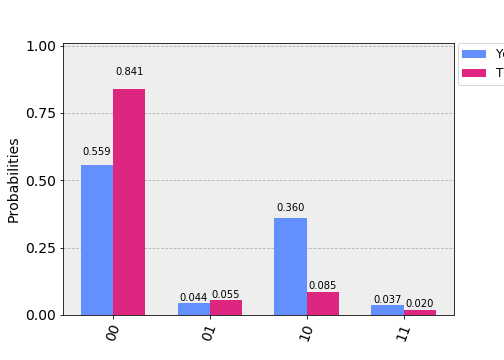
\includegraphics[width=\linewidth]{img/qecc3_X00.png}
      \end{minipage}&
      \begin{minipage}{.215\textwidth}
        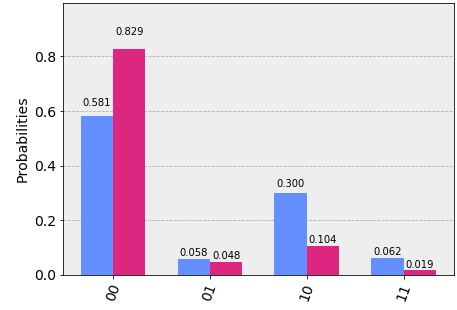
\includegraphics[width=\linewidth]{img/qecc3_Y00.png}
      \end{minipage}
      &\begin{minipage}{.215\textwidth}
        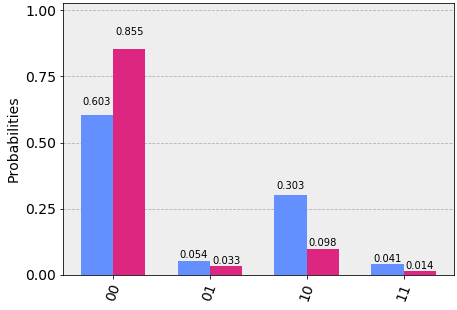
\includegraphics[width=\linewidth]{img/qecc3_Z00.png}
      \end{minipage}
      &\begin{minipage}{.215\textwidth}
        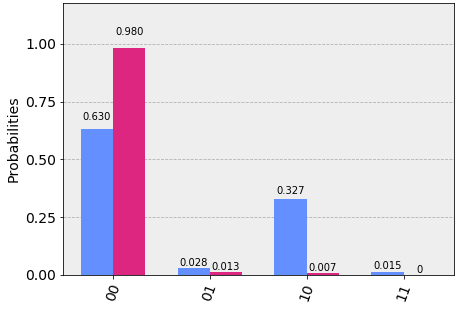
\includegraphics[width=\linewidth]{img/qecc3_I00.png}
      \end{minipage}
      \\ \hline
      01 & 
      \begin{minipage}{.215\textwidth}
        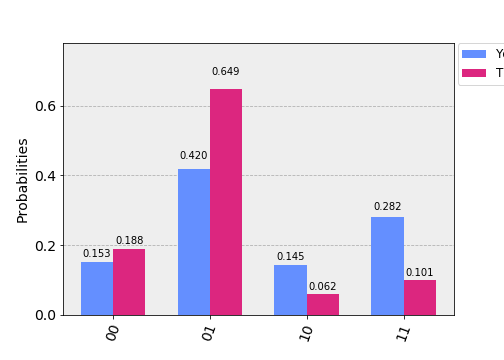
\includegraphics[width=\linewidth]{img/qecc3_X01.png}
      \end{minipage}&
      \begin{minipage}{.215\textwidth}
        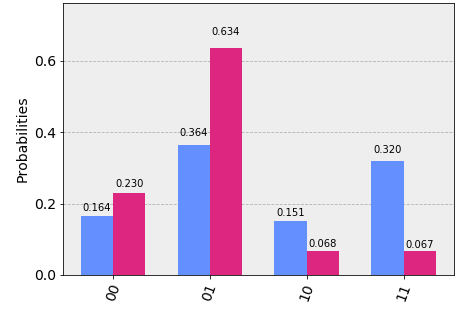
\includegraphics[width=\linewidth]{img/qecc3_Y01.png}
      \end{minipage}
      &\begin{minipage}{.215\textwidth}
        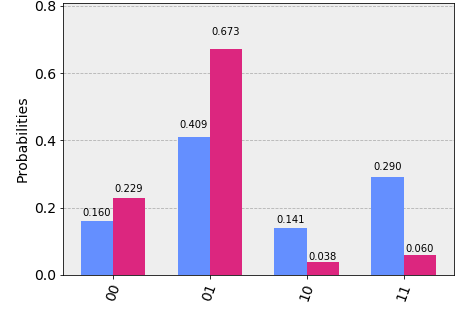
\includegraphics[width=\linewidth]{img/qecc3_Z01.png}
      \end{minipage}
      &\begin{minipage}{.215\textwidth}
        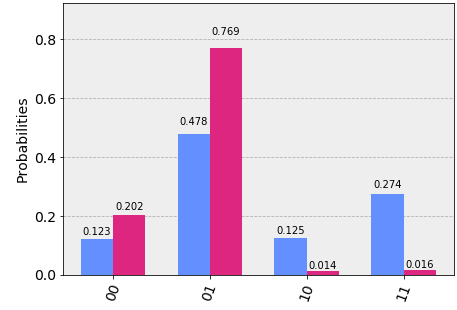
\includegraphics[width=\linewidth]{img/qecc3_I01.png}
      \end{minipage}
      \\ \hline
      10 & 
      \begin{minipage}{.215\textwidth}
        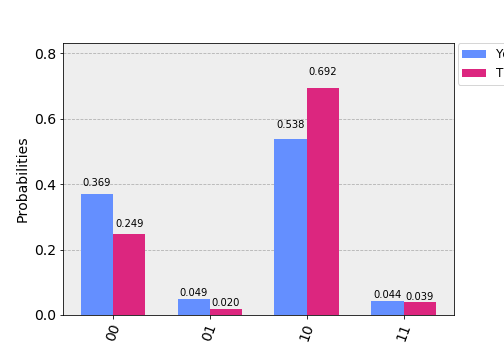
\includegraphics[width=\linewidth]{img/qecc3_X10.png}
      \end{minipage}&
      \begin{minipage}{.215\textwidth}
        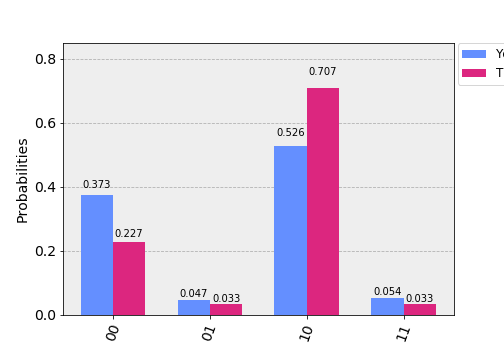
\includegraphics[width=\linewidth]{img/qecc3_Y10.png}
      \end{minipage}
      &\begin{minipage}{.215\textwidth}
        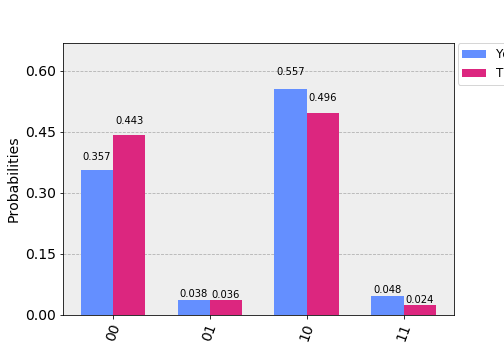
\includegraphics[width=\linewidth]{img/qecc3_Z10.png}
      \end{minipage}
      &\begin{minipage}{.215\textwidth}
        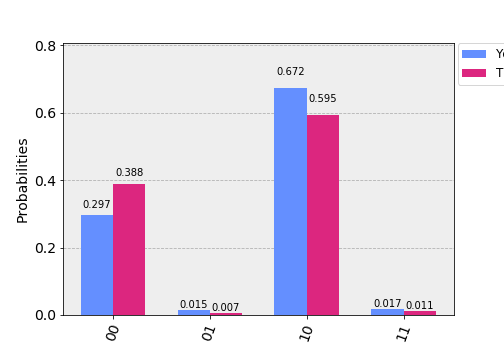
\includegraphics[width=\linewidth]{img/qecc3_I10.png}
      \end{minipage}
      \\ \hline
      11 & 
      \begin{minipage}{.215\textwidth}
        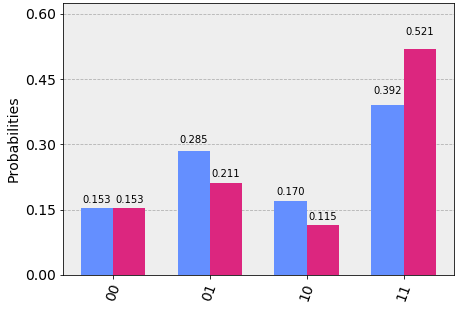
\includegraphics[width=\linewidth]{img/qecc3_X11.png}
      \end{minipage}&
      \begin{minipage}{.215\textwidth}
        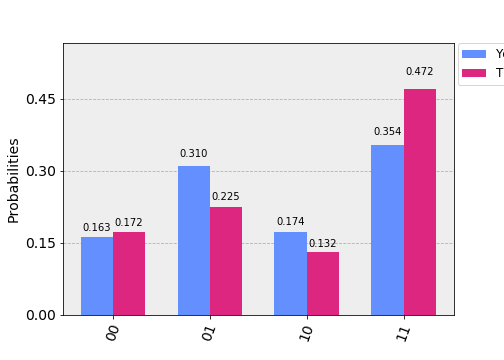
\includegraphics[width=\linewidth]{img/qecc3_Y11.png}
      \end{minipage}
      &\begin{minipage}{.215\textwidth}
        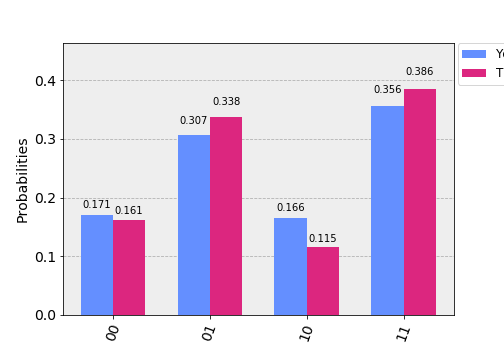
\includegraphics[width=\linewidth]{img/qecc3_Z11.png}
      \end{minipage}
      &\begin{minipage}{.215\textwidth}
        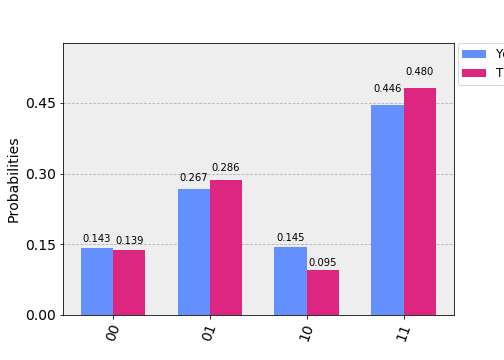
\includegraphics[width=\linewidth]{img/qecc3_I11.png}
      \end{minipage}
      \\ \hline
    \end{tabular}
    \caption{Inputs and Errors on sigma = 0, Legend: Tenerife (pink) and Yorktown (blue)}\label{tbl:sig0}
\end{table}

\begin{table}[h!]
    \centering
    \begin{tabular}{| c | c | c | c | c | }
      \hline
      & X error & Y error & Z error & No error \\ 
      \hline
      00 & 
      \begin{minipage}{.215\textwidth}
        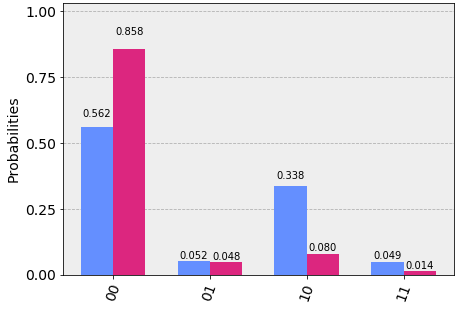
\includegraphics[width=\linewidth]{img/one_qecc3_X00.png}
      \end{minipage}&
      \begin{minipage}{.215\textwidth}
        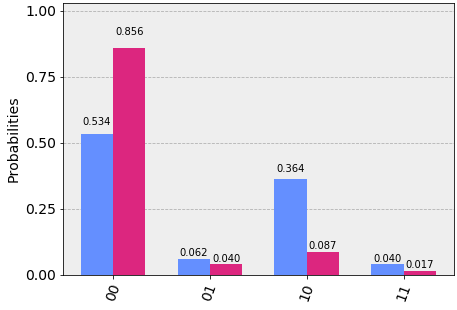
\includegraphics[width=\linewidth]{img/one_qecc3_Y00.png}
      \end{minipage}
      &\begin{minipage}{.215\textwidth}
        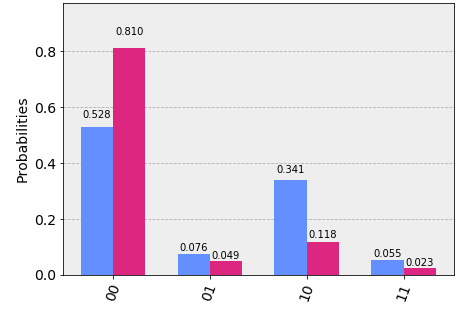
\includegraphics[width=\linewidth]{img/one_qecc3_Z00.png}
      \end{minipage}
      &\begin{minipage}{.215\textwidth}
        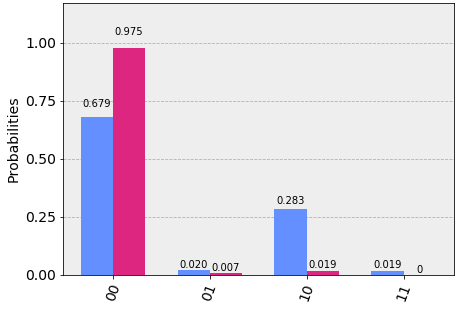
\includegraphics[width=\linewidth]{img/one_qecc3_I00.png}
      \end{minipage}
      \\ \hline
      01 & 
      \begin{minipage}{.215\textwidth}
        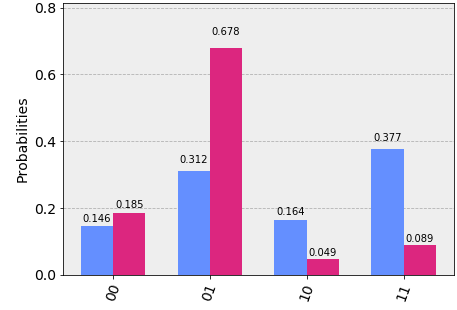
\includegraphics[width=\linewidth]{img/one_qecc3_X01.png}
      \end{minipage}&
      \begin{minipage}{.215\textwidth}
        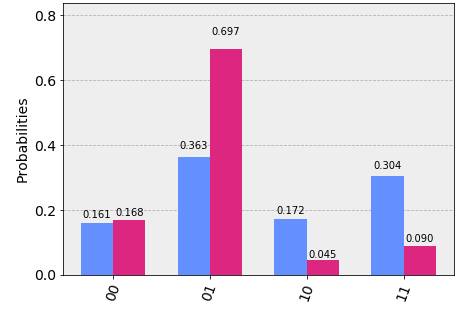
\includegraphics[width=\linewidth]{img/one_qecc3_Y01.png}
      \end{minipage}
      &\begin{minipage}{.215\textwidth}
        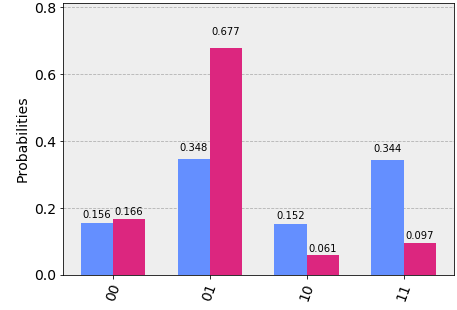
\includegraphics[width=\linewidth]{img/one_qecc3_Z01.png}
      \end{minipage}
      &\begin{minipage}{.215\textwidth}
        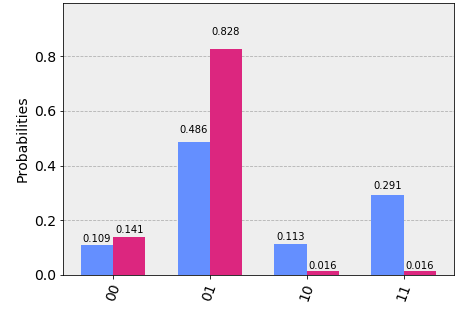
\includegraphics[width=\linewidth]{img/one_qecc3_I01.png}
      \end{minipage}
      \\ \hline
      10 & 
      \begin{minipage}{.215\textwidth}
        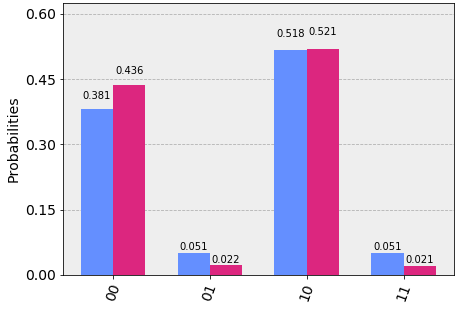
\includegraphics[width=\linewidth]{img/one_qecc3_X10.png}
      \end{minipage}&
      \begin{minipage}{.215\textwidth}
        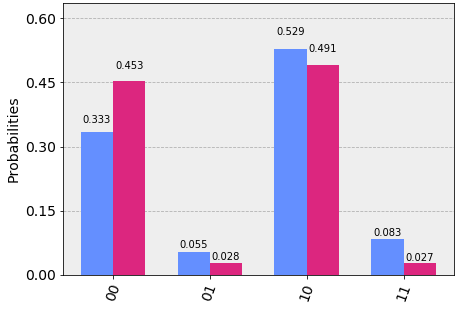
\includegraphics[width=\linewidth]{img/one_qecc3_Y10.png}
      \end{minipage}
      &\begin{minipage}{.215\textwidth}
        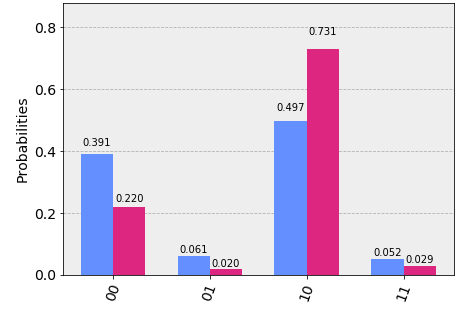
\includegraphics[width=\linewidth]{img/one_qecc3_Z10.png}
      \end{minipage}
      &\begin{minipage}{.215\textwidth}
        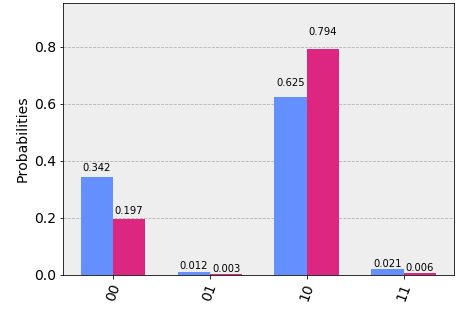
\includegraphics[width=\linewidth]{img/one_qecc3_I10.png}
      \end{minipage}
      \\ \hline
      11 & 
      \begin{minipage}{.215\textwidth}
        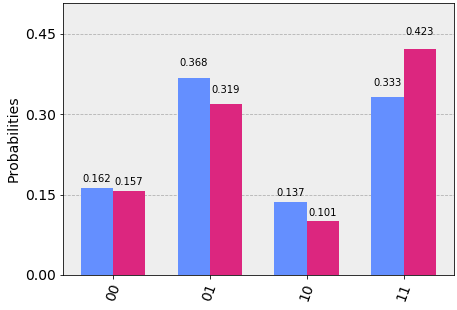
\includegraphics[width=\linewidth]{img/one_qecc3_X11.png}
      \end{minipage}&
      \begin{minipage}{.215\textwidth}
        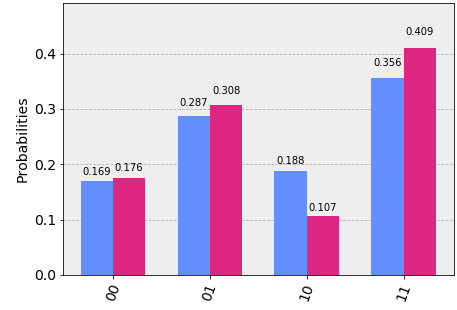
\includegraphics[width=\linewidth]{img/one_qecc3_Y11.png}
      \end{minipage}
      &\begin{minipage}{.215\textwidth}
        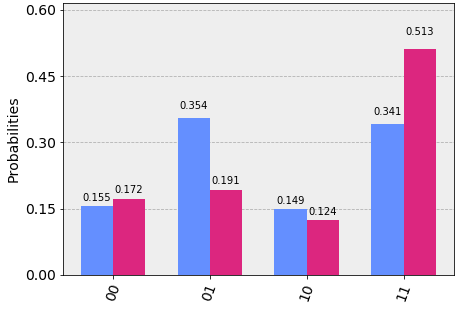
\includegraphics[width=\linewidth]{img/one_qecc3_Z11.png}
      \end{minipage}
      &\begin{minipage}{.215\textwidth}
        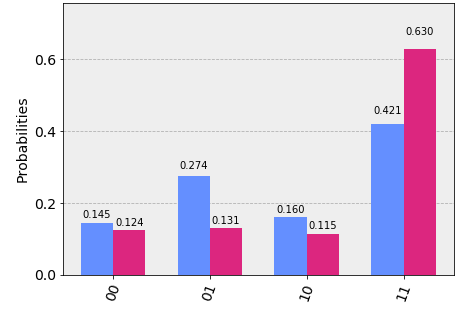
\includegraphics[width=\linewidth]{img/one_qecc3_I11.png}
      \end{minipage}
      \\ \hline
    \end{tabular}
    \caption{Inputs and Errors on sigma = 1, Legend: Tenerife (pink) and Yorktown (blue)}\label{tbl:sig1}
  \end{table}

\begin{table}[h!]
\centering
\begin{tabular}{| c | c | c | c | c | }
    \hline
    & X error & Y error & Z error & No error \\ 
    \hline
    00 & 
    \begin{minipage}{.215\textwidth}
    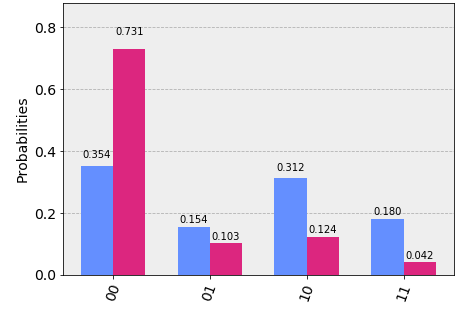
\includegraphics[width=\linewidth]{img/rand_qecc3_X00.png}
    \end{minipage}&
    \begin{minipage}{.215\textwidth}
    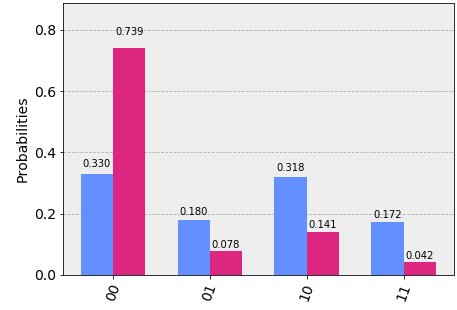
\includegraphics[width=\linewidth]{img/rand_qecc3_Y00.png}
    \end{minipage}
    &\begin{minipage}{.215\textwidth}
    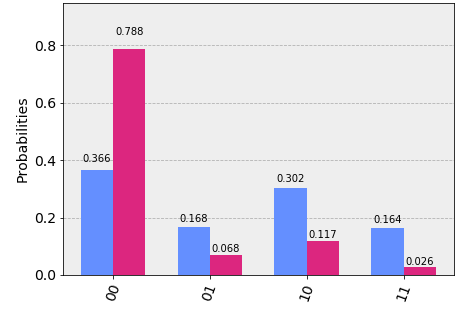
\includegraphics[width=\linewidth]{img/rand_qecc3_Z00.png}
    \end{minipage}
    &\begin{minipage}{.215\textwidth}
    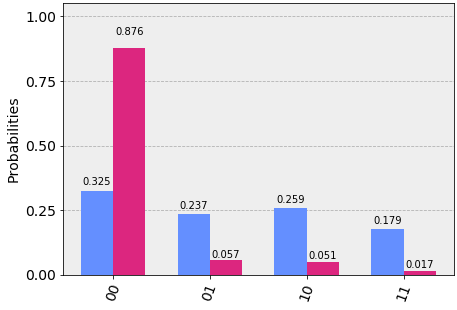
\includegraphics[width=\linewidth]{img/rand_qecc3_I00.png}
    \end{minipage}
    \\ \hline
    01 & 
    \begin{minipage}{.215\textwidth}
    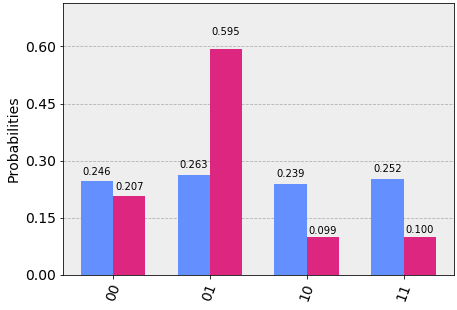
\includegraphics[width=\linewidth]{img/rand_qecc3_X01.png}
    \end{minipage}&
    \begin{minipage}{.215\textwidth}
    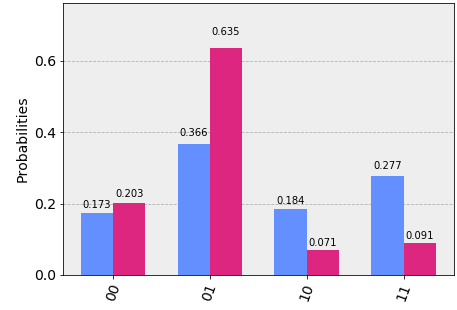
\includegraphics[width=\linewidth]{img/rand_qecc3_Y01.png}
    \end{minipage}
    &\begin{minipage}{.215\textwidth}
    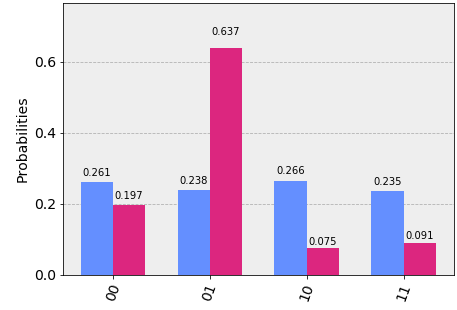
\includegraphics[width=\linewidth]{img/rand_qecc3_Z01.png}
    \end{minipage}
    &\begin{minipage}{.215\textwidth}
    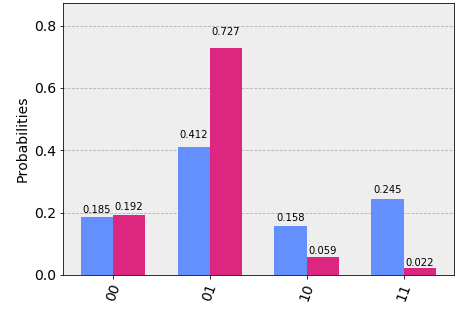
\includegraphics[width=\linewidth]{img/rand_qecc3_I01.png}
    \end{minipage}
    \\ \hline
    10 & 
    \begin{minipage}{.215\textwidth}
    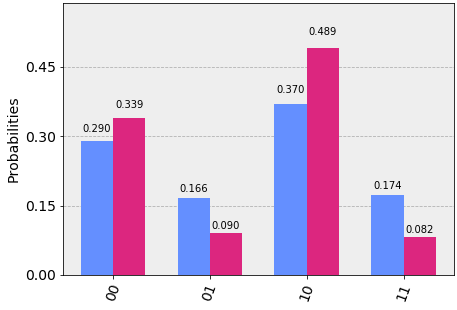
\includegraphics[width=\linewidth]{img/rand_qecc3_X10.png}
    \end{minipage}&
    \begin{minipage}{.215\textwidth}
    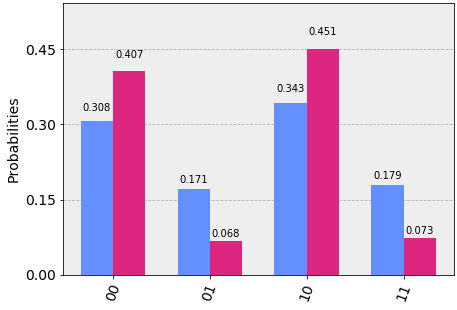
\includegraphics[width=\linewidth]{img/rand_qecc3_Y10.png}
    \end{minipage}
    &\begin{minipage}{.215\textwidth}
    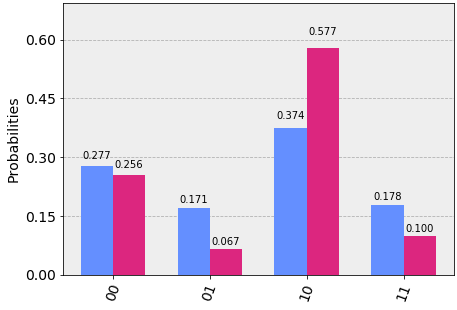
\includegraphics[width=\linewidth]{img/rand_qecc3_Z10.png}
    \end{minipage}
    &\begin{minipage}{.215\textwidth}
    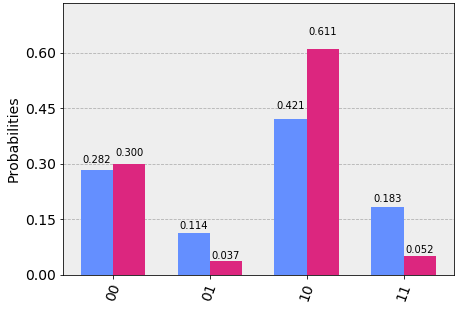
\includegraphics[width=\linewidth]{img/rand_qecc3_I10.png}
    \end{minipage}
    \\ \hline
    11 & 
    \begin{minipage}{.215\textwidth}
    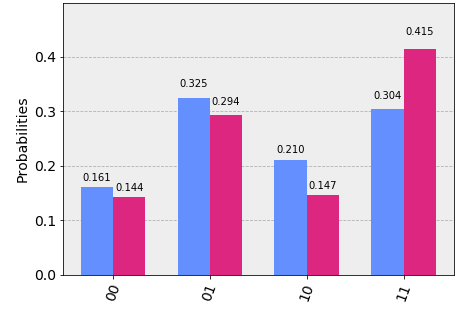
\includegraphics[width=\linewidth]{img/rand_qecc3_X11.png}
    \end{minipage}&
    \begin{minipage}{.215\textwidth}
    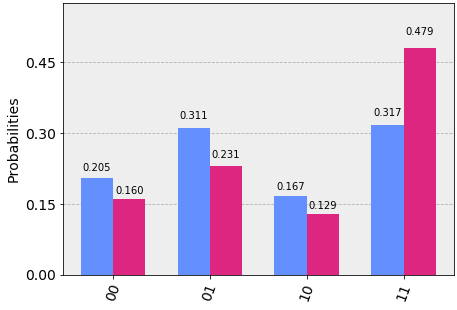
\includegraphics[width=\linewidth]{img/rand_qecc3_Y11.png}
    \end{minipage}
    &\begin{minipage}{.215\textwidth}
    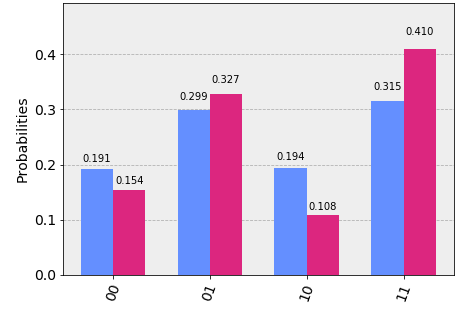
\includegraphics[width=\linewidth]{img/rand_qecc3_Z11.png}
    \end{minipage}
    &\begin{minipage}{.215\textwidth}
    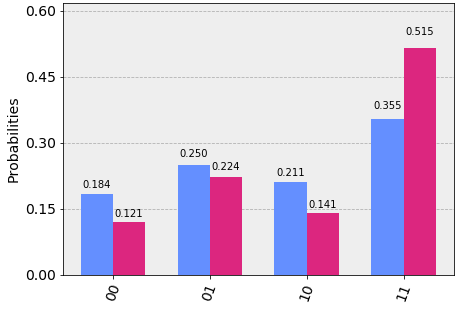
\includegraphics[width=\linewidth]{img/rand_qecc3_I11.png}
    \end{minipage}
    \\ \hline
\end{tabular}
\caption{Inputs and Errors on random sigma, Legend: Tenerife (pink) and Yorktown (blue)}\label{tbl:sigR}
\end{table}

We can test the encoding scheme on $\ket{0000}$ and $\ket{00000}$, as shown in Figure \ref{fig:q45}. In the case of 4 qubits, Tenerife finds the correct output, but neither computer has fidelity in the 5 qubit case. 

\begin{figure}[h!]
\centering
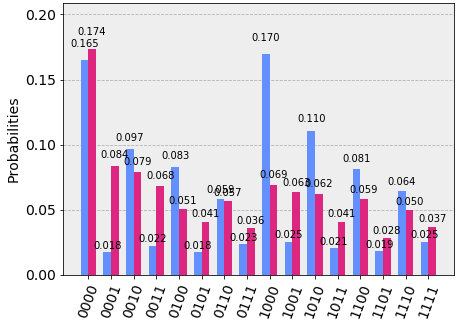
\includegraphics[width=.45\textwidth]{img/qecc4_X0000.png}
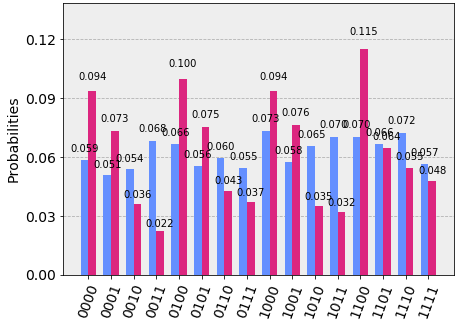
\includegraphics[width=.45\textwidth]{img/qecc5_X00000.png}
\caption{QECC on 4 and 5 qubits}
\label{fig:q45}
\end{figure}
\end{document}

